%% This is an example first chapter.  You should put chapter/appendix that you
%% write into a separate file, and add a line \include{yourfilename} to
%% main.tex, where `yourfilename.tex' is the name of the chapter/appendix file.
%% You can process specific files by typing their names in at the 
%% \files=
%% prompt when you run the file main.tex through LaTeX.
\chapter{Background}
\section{Preface}
Gravitational wave astronomy is often called a new way of observing the universe, partly due to the recent nature of its confirmation through direct observation. The reality of the situation is that the 2015 detection of GWs was made possible only through the careful and determined efforts of the LIGO and VIRGO scientific collaborations, which consist of thousands of scientists whose work spans decades. The motivation for this comes from theoretical work that is traceable back to Einstein himself and the original theoretical prediction of gravitational waves as a mathematical consequence of general relativity. As a result the theory as well as the methods and techniques in practical use in Advanced LIGO era are highly mature and developed and perhaps somewhat subtle to those not directly familiar with GW signal processing and data analysis. The purpose of this chapter is to provide a brief overview of these techniques to both remind the experienced researcher of why we use the processes we use, as well as introduce the more general scientific audience to the basics of GW physics and astronomy as it pertains to this work. We present an overview of the theory of linearized gravity starting (and ending) with the Einstein field equations. We introduce Bayesian statistics as our main tool for analysis and connect it to our work, hopefully providing enough foundation to elucidate our choices and motivations for completing this work.  

\section{The Einstein Field Equation}
The Einstein Field Equations are the central objects of study in General Relativity. They are ten, coupled, nonlinear, partial differential equations in four dimensions. They are the following:

\begin{align}\label{eq:fulleinst}
R_{\mu \nu} - \frac{1}{2}Rg_{\mu \nu} = T_{\mu \nu}
\end{align}

Just as a differential equation relates the forces and constraints in a physical system to, perhaps, a function (and its derivatives) describing the motion of a particle through space and time, the Einstein field equations relate the mass and energy in a region of spacetime to the \textit{metric tensor} $g_{\mu \nu}$ and its derivatives, from which the geodesic paths objects follow through space and time can be derived. In this way $g_{\mu \nu}$ itself can be viewed as a \textit{solution} to the field equations given some sources or sinks in the region in question. In the following sections we will briefly motivate the pieces of the equation itself and hopefully provide some basic intuition as to how Einstein wrote this relationship down, and how from it we may mathematically derive the existence of gravitational waves in their entirety. 

\subsection{Reimann Tensor}
The Reimann Tensor is a mathematical object that encapsulates the geometric \textit{curvature} of spacetime. The concept of a curved spacetime is fundamentally no different from the concept of a curved space, and from examining the behavior of vectors in such a space we can address both the purpose and properties of the Reimann tensor without departing from the intuitive picture of spheres and arrows.

\begin{figure}[h!]\label{fig:reimann}
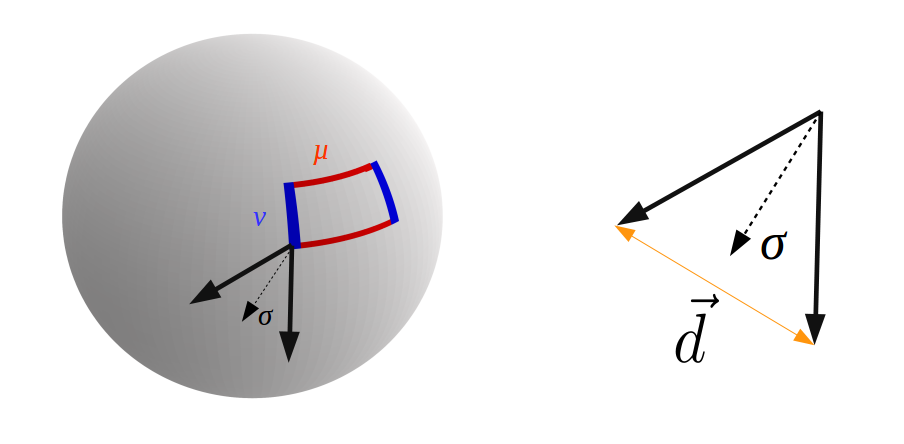
\includegraphics[scale=0.5]{reimann.png}
\caption{A visual depiction of the Reimann Curvature tensor. Parallel transporting a vector originally pointing in the $\sigma$ direction both ways around the loop shown yields two different vectors. The orange vector $\vec{d}$ points between the tips. The magnitude of the components of this vector are $R_{\rho \sigma \mu \nu}$.} The first symmetry of the Reimann tensor is apparent - interchanging the last two indices would simply yield the same vector $\vec{d}$ the the opposite sign on all the components.
\label{fig:sphere}
\end{figure}

The Reimann tensor is traditionally derived by examining the local behavior of geodesics subject to a metric tensor that describes curved space. Here we motivate the concept with a visual explanation of parallel transport. Consider a vector pointing in some arbitrary direction $\sigma$ somewhere on the sphere, as depicted in figure \ref{fig:sphere}. If we maintain the orientation of the vector relative to the surface of the sphere as we traverse the path, we note that the vector behaves differently depending on the order in which we choose to traverse the directions $\mu$ and $\nu$. This difference is representable by a vector that points between the two tips - one that is dependent on the initial direction $\sigma$ and both the transport directions $\mu$ and $\nu$. Let this vector be denoted $\vec{d}$. Then the Reimann tensor, $R_{\rho \sigma \mu \nu}$, is simply $d_{\rho}$, the $\rho$'th component of this difference vector. From this geometric picture some of the classical symmetries that are often introduced abreast the definition of the Reimann tensor are immediately intuitive, such as the skew symmetry depicted in figure \ref{fig:reimann}.
Since it is somewhat unfair (worse - \textit{incorrect}) to characterize the entire geometry of the space with looping paths over large areas, the formal definition of the Reimann tensor is in fact the infinitesimal version of the concept above. It is sometimes written as 

\begin{align}
R^{\rho}_{\sigma \mu \nu}\partial_{\rho} = \left(\nabla_{\mu}\nabla{\nu} - \nabla_{\nu}\nabla_{\mu}\right)\partial_{\sigma}
\end{align} 

It should be noted that the above formula is true only modulo a term containing $\nabla_{[\mu, \nu]}$ except in the special case of coordinate vector fields, where it is zero. This also illuminates why the Reimann tensor is sometimes described as encoding the non-commutativity of covariant derivatives on a manifold. Crucial to a straightforward linearization of the Reimann tensor itself is the expression in terms of the Christoffel symbols defined in \nameref{Appendix C}. 

\begin{align}\label{eq:reimanntnsfull}
R^{\rho}_{\sigma \mu \nu} = \partial_{\mu}\Gamma^{\rho}_{\nu \sigma} - \partial_{\nu}\Gamma^{\rho}_{\mu \sigma} + \Gamma^{\rho}_{\mu \lambda}\Gamma^{\lambda}_{\nu \sigma} - \Gamma^{\rho}_{\nu \lambda}\Gamma^{\lambda}_{\mu \sigma}
\end{align}

\subsection{Ricci Tensor}

Some experimentation with various contractions of the Reimann tensor as defined by equation \ref{eq:reimanntnsfull} over its own indices reveals that there is only one nonzero result:

\begin{align}
R_{\mu \nu} &\equiv R^\alpha_{\sigma \alpha \nu}
\end{align} 

This is called the Ricci Tensor and represents the full trace of the Reimann tensor. Einstein's equaiton provides the only means to a physical interpretation of this result. Under the assumption that equation \textbf{EINSTEIN} is the correct relation between spacetime curvature and local sources, then the traceless remnant of the Reimann tensor must describe the spacetime curvature from \textit{external} sources. This is named the Weyl tensor and it plays an important role in describing the propagation of gravitational radiation. Indeed, a spacetime carrying gravitational radiation may satisfy the vacuum Einstein equation 

\begin{align}
R_{\mu \nu} = 0
\end{align}

But may \textit{not} satisfy
\begin{align}
R^\rho_{\sigma \mu \nu} = 0
\end{align}

\subsection{Ricci Scalar}

The most natural line of logic to pursue next is what happens when the Ricci tensor itself is contracted over the two remaining indices. 

\begin{align}
R \equiv R^{\alpha}_{\alpha} = g^{\mu \nu}R_{\mu \nu}
\end{align}

The result is the Ricci scalar of scalar curvature which is a unique scalar measuring the local curvature at every point on the manifold. It is only one of many ways of assigning a scalar to each point, and geometrically it is the average of the Gaussian curvatures for all two dimensional "cross sections" that exist within the tangent space at the point in question.  

\subsection{Stress-Energy-Momentum Tensor}
It is the opinion of the author that the motivations behind why the stress-energy-momentum tensor falls on the right hand side of equation \ref{eq:fulleinst} are best understood by following the same line of logic taken historically by Einstein, Minkowski and Von Laue. This discussion has been relegated to Appendix A. For now it will suffice to say that $T_{\mu \nu}$ reconciles what was in the early 1900s the new formalism of four-vectors with fundamental concepts such as the continuity equation. It bridged the gap between the mature machinery of relativistic electric and magnetic fields and "other" types of matter, casting them as one in the same. For now we will simply say that it may be found by considering the properties of matter and energy in a region and plays the role of the source term in equation \ref{eq:fulleinst}.   

\section{Linearization}

In linearized gravity we assume the spacetime is described by a flat spacetime $g_{\mu \nu}$ plus a small perturbation

\begin{align}\label{eq:metpluspert}
g_{\mu \nu} = \eta_{\mu \nu} + h_{\mu \nu}
\end{align}

Since the other pieces of the Einstein field equations are directly derived from the metric, they must be individually linearized to form a description of spacetime around weak sources. The standard treatment of linearized gravity assumes that to first order we may raise and lower indices using the Minkowski metric.

\begin{align}
h^\mu_\nu = \eta^{\alpha \mu} h_{\alpha \nu} \ \  \text{and} \ \ h^{\mu \nu} = \eta^{\alpha \mu}\eta^{\beta \nu}h_{\alpha \beta}
\end{align}

While the details steps are expanded in Appendix C, we state here without proof that the following statements are true. The next natural line of logic to pursue is to write down the Christoffel symbols for such a spacetime

\begin{align}
\Gamma^{\mu}_{\alpha \beta} &= \frac{1}{2} \left[\partial_{\beta} h^{\mu}_{\alpha} + \partial_{\alpha}h_{\beta}^{\mu} - \partial^{\mu}h_{\alpha \beta}\right] 
\end{align}

These can be used to define the linearized Reimann and Ricci tensors along with the Ricci scalar:

\begin{align}
R^{\rho}_{\sigma \mu \nu} &= \partial_{\mu}\Gamma^{\rho}_{\nu \sigma} - \partial_{\nu}\Gamma^{\rho}_{\mu \sigma} \\ 
R_{\mu \nu} &= \frac{1}{2}\left[\partial_{\alpha}\partial_{\mu}h^{\alpha}_{\nu} + \partial_{\nu}\partial^{\alpha}h_{\mu \alpha} - \partial_{\alpha}\partial^{\alpha}h_{\mu \nu} - \partial_{\nu}\partial_{\mu}h^{\alpha}_{\alpha}\right] \\ \label{eq:linricci} 
R &= \partial_{\alpha}\partial_{\mu}h^{\mu \alpha} - \Box h
\end{align}

With the linearized Reimann tensor in hand, it turns out through various gauge freedoms and coordinate transformations also expounded upon in the appendix that the linearized, vacuum Einstein field equation is simply 

\begin{align}\label{eq:flteinst}
\Box h_{\mu \nu} = 0
\end{align}

Which is a wave equation in the tensor purturbation's components. The same freedoms serve to reveal that out of the sixteen wave equations that correspond to equation \ref{eq:flteinst}, only two are physically meaningful. Orienting the coordinate frame such that the wave propagation direction lies along the $z$ axis, these two degrees of freedom are manifest as the $x$ and $y$ spatial distortions

\begin{align}
h_{\mu \nu} = 
\begin{bmatrix}
0 & 0 & 0 & 0 \\
0 & h_+ & h_\times & 0 \\
0 & h_\times & -h_+ & 0 \\
0 & 0 & 0 & 0
\end{bmatrix}
\end{align}  

In which the $+$ and $\times$ "polarizations" of the spatially propagating tensor disturbance satisfy

\begin{align}
h_p(\vec{x}) = A_p e^{i \mathbf{k}\cdot\mathbf{x}}
\end{align}

It will be convenient in the coming chapters to define the gravitational wave strain in a detector $h(t)$ subject to this disturbance to this disturbance as single complex number that encodes these two independent degrees of freedom as one object:

\begin{align}
h(t) = h_+(t) - i h_{\times}(t)
\end{align}

\section{Bayesian Statistics}

We select a Bayesian posterior probability as our main analysis technique as its ability to quantify and propagate uncertainties in parameter estimates is well documented \cite{Volume-2} as a tool of choice for gravitational wave signal processing. Bayes' Theorem follows from the symmetric definition of conditional probability depicted visually in figure \ref{fig:distrib}. Let the joint probability evaluated at any point $(x,y)$ in the plane be denoted $P(x,y)$. We may take a cross section through the joint probability distribution along any direction we choose, let us call such a cross section parallel to the $x$ axis the conditional probability of $x$ given $y$, and denote it $P(x|y)$. A perpandicular cross section would simply be $P(y|x)$. We see that we can compute $P(x,y)$ in two equivalent ways: scaling $P(x|y)$ by $P(y)$ or by scaling $P(y|x)$ by $P(x)$. Thus we have that 


\begin{figure}[h!]
\center
\includegraphics[trim={1cm, 1cm, 1cm, 1cm}, clip]{biviariate_norm_done.eps}
\caption{A joint probability distribution $P(x,y)$. The contours parallel with the $x$ direction represent different $P(y|x)$.}
\label{fig:sphere}
\end{figure}

\begin{align} \label{eq:bayes}
P(x|y)P(y) &= P(y|x)P(x) \\
P(x|y) &= \frac{P(y|x)P(x)}{P(y)}
\end{align}

Which is Bayes' theorem. The denominator of the expression on the right hand side is often rewritten as a sum over all possible situations in which $y$ is an outcome. Reading $\neg x$ as "not x", we have

\begin{align}\label{eq:continuous}
P(y) &= P(y|x)P(x) + P(y|\neg x)P(\neg x) \\
&= \sum_{k=1}^K P(y|x_k)P(x_k) 
\end{align}


\clearpage 
This allows us to rewrite the posterior probability as

\begin{align}
P(x|y) = \frac{P(y|x) P(x)}{\sum_{k=1}^K P(y|x_k)P(x_k)}
\end{align}

Multiplying the right hand side of this equation by the quantity $\frac{1}{P(x)P(y|\neg x)}$ one has 

\begin{align} \label{eq:lratio}
P(x|y) &= \frac{\Lambda(x|y)}{\Lambda(x|y) + \frac{P(\neg x)}{P(x)}}
\end{align}

Where we have used the \textit{likelihood ratio} $\Lambda(x|y) \equiv \frac{P(y|x)}{P(y|\neg x)}$ to simplify the expression. The likelihood ratio has a simple interpretation, it is simply the ratio of the probability of event $y$ occuring in the case event $x$ occurs and the probability of event $y$ occuring given that event $x$ \textit{does not} occur. In fact, this form of Bayes theorem indicates that the posterior probability for $x$ given $y$ is directly proportional to the likelihood ratio. This is particularly important in the Bayesian treatment of gravitational waves where the central question for study is the probability of observing the data in question given that there may or may not be a signal present.  

\subsection{Signal Processing}
Noise in the LIGO detectors is modeled as \textit{Gaussian Noise}, which describes a length $N$ set of time series samples $\{x_j\}$ with the following probability of observation:

\begin{align}
P(\{x_j\}) = \left[\frac{1}{\sqrt{2 \pi} \sigma}\right]^N e^{-\frac{1}{2 \sigma^2} \sum_{j = 0}^{N - 1}x_j^2}
\end{align}

If we allow the $\{x_j\}$ to be weighted by the noise sensitivity in frequency space (also known as the \textit{power spectral density}) $S(f) = \sum_{k=0}^K n^*(f_k)n(f_k) \equiv \braket{n(f)|n(f)}$ then we may write the probability density for any Gaussian noise process as 

\begin{align}
P_x(\{x(t)\}) \propto e^{-\frac{1}{2}\braket{x(t)|x(t)}}
\end{align}

For gravitational wave signal processing we are interested in evaluating the equivalent of the likelihood ratio  in equation \ref{eq:lratio} for the null and signal present hypotheses, $\mathcal{H}_0$ and $\mathcal{H}_1$ respectively. Following the treatment outlined in literature \cite{rapidpe} This is

\begin{align}
\Lambda(\mathcal{H}_1|d) &= \frac{P(d|\mathcal{H}_1)}{P(d|\mathcal{H}_0)}
\end{align}

In the above equation $\mathcal{H}_0$ is in direct correspondence with $\neg x$ and $\mathcal{H}_1$ is in direct correspondence with $x$. If there is no signal present in the data, then the data and noise are equal, meaning 

\begin{align}
d(t) &= n(t) \\
P(d(t)|\mathcal{H}_0) &\propto e^{-\frac{1}{2}\braket{d(t)|d(t)}}
\end{align} 

Whereas if there is a signal present in the data, then the noise is the \textit{residual} signal after the gravitational wave potion of the signal $h(t)$ is subtracted from the total signal $d(t)$: 

\begin{align}
d(t) &= n(t) + h(t) \\
p(d(t)|\mathcal{H}_1) &\propto e^{-\frac{1}{2}\braket{d(t) - h(t)|d(t) - h(t)}}
\end{align}

So the likelihood ratio for gravitational wave signal processing is exactly equal to 

\begin{align}
\Lambda(\mathcal{H}_1|d(t)) &= \frac{e^{-\frac{1}{2}\braket{h(t)-d(t)|h(t)-d(t)}}}{e^{-\frac{1}{2}\braket{d(t)|d(t)}}}
\end{align}

By equation \ref{eq:bayes}  the posterior probability of a gravitational wave signal with parameters $\mu$ is given by 

\begin{align}\label{eq:parampos}
P[\vec{\mu}, \mathcal{H}_1|d(t)] = \frac{P[d(t)|\vec{\mu}, \mathcal{H}_1]P(\vec{\mu})}{P[d(t), \mathcal{H}_1]}
\end{align}

Extending equation \ref{eq:continuous} to the case of a continuous state space we have for the denominator

\begin{align}
P[d(t), \mathcal{H}_1] &= \int_{\Omega}P[d(t)|\vec{\mu}, \mathcal{H}_1]P(\vec{\mu})d\vec{\mu}
\end{align}

Where $\Omega$ indicates integration over the entire probabilistic state space. Dividing both the top and bottom of the right hand side of equation \ref{eq:parampos} by $P(d(t)|\vec{\mu}, \mathcal{H}_1)$ gives us 

\begin{align}\label{eq:bayeslikely}
P(\vec{\mu}, \mathcal{H}_1|d(t)) = \frac{\Lambda(d(t)|\vec{\mu}, \mathcal{H}_1)P(\vec{\mu})}{\int_{\Omega}\Lambda(d(t)|\vec{\mu}, \mathcal{H}_1)P(\vec{\mu})d\vec{\mu}}
\end{align}

Note that the integral in the denominator may be factored into components that are functions of independent groups of parameters. For the purposes of gravitational wave data analysis it is factored into intrinsic and extrinsic parameters, the former (masses, spins) being responsible for the actual orbital dynamics of the system, and the latter (distance, inclination, right ascension, declination) depending only on the nature of the observer relative to the source. We label these sets of paramters $\vec{\lambda}$ and $\vec{\theta}$ respectively. The denominator of equation \ref{eq:bayeslikely} is thus factorizable as 

\begin{align}
\int_{\Omega}\Lambda(d(t)|\vec{\mu}, \mathcal{H}_1)d\vec{\mu} &= \int_{\Omega}\Lambda(d(t)|\vec{\lambda}, \mathcal{H}_1)P(\vec{\lambda})d\vec{\lambda}\int_{\Omega}\Lambda(d(t)|\vec{\theta}, \mathcal{H}_1)P(\vec{\theta})d\vec{\theta} 
\end{align} 

Note that while evaluating the likelihood for a single set of parameters in the numerator of the above equation may not be any serious challenge, computing the integral in the denominator is. Many schemes \cite{rapidpe} \cite{lalinference} \cite{mcmc} have been developed to tackle this particular problem and generally involve simulating the posterior through MCMC sampling. These techniques are highly developed and at the time of writing can provide converged results on the order of days, however they are limited in their parallelism due fundamental serialization of the algorithm. Cutting edge implementations involving parallel tempering and some forms of ensemble MCMC have shown promising results, however none can take advantage of the many thousands of cores availble across the LIGO data grid. Methods that can scale out to the computational resources provided by the LIGO data grid are needed to reduce runtimes to minutes or less.   

\subsection{Harmonic Mode Decomposition}

For a single detector $k$ We can write our gravitational wave signal $h_k(t) = h_{+,k}(t) - ih_{\times, k}(t)$ as a sum over products of harmonic mode strain values $h_{l,m}(\vec{\lambda})$ and corresponding spin-weighted spherical harmonics, scaled by the reference distance and antenna factor:

\begin{align}
h_k(t) = \frac{D_r}{D}F_k(\theta)\sum_{(l,m)}h_{k, (l,m)}(t, \vec{\lambda})Y_{(l,m)}(\vec{\theta})
\end{align}

Where $D_r$ is the luminosity reference distance to the binary. This is defined similarly to the manner in which apparent magnitude is defined versus absolute magnitude in astonomy. We substitute this expression for the signal into the expression for the likelihood ratio we find, taking the logarithm, that

\begin{align}
\mathcal{L} &= \prod_k e^{-\frac{1}{2}\braket{d - h_k|d-h_k} + \braket{d|d}} \\
\ln\mathcal{L} &= -\frac{1}{2}\sum_{k}\left[\braket{d - h_k|d-h_k} + \braket{d|d}\right] \\
&= \frac{1}{2}\sum_{k}\left[-\cancel{\braket{d|d}}+\braket{d|h_k}+\braket{h_k|d}+\braket{h_k|h_k} + \cancel{\braket{d|d}}\right] \\
\end{align}

Now, since for complex vector spaces $\braket{a|b} = \braket{b|a}*$, we have that $\braket{d|h_k} + \braket{h_k|d} = 2\Re\braket{h_k|d}$. Then, 

\begin{align}
\ln\mathcal{L} &= \frac{1}{2}\sum_{k}\left[2\braket{h_k|d} + \braket{h_k|h_k}\right] \\
&= \frac{1}{2} \sum_{k}\Re\left[\braket{2\frac{D_r}{D}F_k(\vec{\theta})\sum_{(l,m)}h_{k,(l,m)}(\lambda)Y_{(l,m)}(\vec{\theta})|d}\right] \\
&+ \left[\frac{D_r}{D}\right]^2F_k^2(\vec{\theta})\sum_{(l,m),(l',m')}h^*_{(l,m)}(\vec{\lambda})h_{(l',m')}(\vec{\lambda})Y^*_{(l,m)}(\vec{\theta})Y_{(l',m')}(\vec{\theta})
\end{align}  

Now, for any complex number $z = a + ib$, we have that $z*z + \Re(z^2) = 2z*z$, so $z*z = \frac{1}{2}(z*z + \Re z^2)$. Then the double sum over $l,m$ pairs becomes




The defining feature of this form of the likelihood is the separation between intrinsic and extrinsic parameters. The intrinsic parameters of the binary exist only within the $h_{k,(l,m)}$, whereas the parameters that depend on the observer are contained entirely within the antenna factor and spherical harmonics. Work by \cite{rapidpe} (RapidPE) has shown that this can be exploited to accelerate computation of the likelihood by precomputing the orbital dynamics of the binary and marginalizing over the extrinsic parameters. The same work computes the posterior over the \textit{intrinsic} parameter space by spreading a grid of points across the $\mathcal{M}, \eta$ plane and computing the integral at each such point, since each of these integrations is independent each point for which the value of the posterior is desired may be assigned its own computational resources. This enables the necessary scaling - the posterior between the points is simply interpolated after all the cores are done. 

\subsection{Precessional Effects}
This work aims to extend and accelerate the ability for RapidPE to estimate gravitational wave parameters. RapidPE is written in Python, and prior to this work significant attention was given to code optimization to obtain the maximum performance possible through Python. Since the terms of the likelihood that may be precomputed involve computationally expensive fourier transforms, calculation of the cross terms $V$ were approximated using the properties of fourier transform to relate 


